\documentclass[a4paper, 12pt]{article}

\newcommand\tab[1][.6cm]{\hspace*{#1}}
\usepackage[portuges]{babel}
\usepackage[utf8]{inputenc}
\usepackage{amsmath}
\usepackage{indentfirst}
\usepackage{graphicx}
\usepackage{multicol,lipsum}
\usepackage{blindtext}
\usepackage{verbatim}
\usepackage{textcomp}
\usepackage{hyperref}
\usepackage{float}
\usepackage{url}

\begin{document}

\begin{titlepage}
	\begin{center}
	
	\begin{figure}[ht]
    \centering
    
\includegraphics[width=.44\textwidth]{Images/LogoUFSJ.PNG}
    \label{fig:Capturar.PNG}
    \end{figure}

    	\Huge{Universidade Federal São João del Rei}\\
		\Large{Departamento de Ciência da Computação}\\ 

        \vspace{110pt}
        \textbf{\LARGE{
        \\
        \\
        \\
        Trabalho Prático 4: Documentação\\
        \vspace{0.5cm}
        \Large{Inteligência Artificial}
        \\
        \\
        \\
        }}
        
		\title{{\large{Título}}}
		\vspace{1cm}
	\end{center}
	    
    \begin{flushleft}
		\begin{tabbing}
		\\
		\\
		\\	
		\large{Alunos: Elias de Paula Pereira,}\\ 
		\large{\hspace{1.9cm}Mariane Rodrigues Costa e}\\
		\large{\hspace{1.9cm}Julio Cesar da Silva Rodrigues}
		\\
	    \\
		\large{Professor: Diego Roberto Colombo Dias}\\
	    \end{tabbing}
    \end{flushleft}
	\vspace{0.85cm}
	
	\begin{center}
		\vspace{\fill}
			Julho\\
		    2022
	\end{center}
\end{titlepage}

\tableofcontents
\newpage

\section{Introdução}

Neste documento, encontram-se os detalhes considerados mais relevantes no desenvolvimento de dois tipos de redes neurais (DNN e CNN) como modelos de aprendizado de máquina para o reconhecimento de dígitos manuscritos. A implementação foi realizada utilizando linguagem Python com auxílio dos recursos do \emph{framework} \textbf{TensorFlow} e os \emph{scripts} presentes na especifcação do trabalho prático, e está disponível publicamente no seguinte endereço \url{https://colab.research.google.com/github/juliorodrigues07/manuscript_digit_recognition/blob/master/cnn_digit.ipynb} no formato \emph{notebook}, e também no repositório \url{https://github.com/juliorodrigues07/manuscript_digit_recognition}.

Antes de prosseguir, vale a pena citar que a DNN foi implementada apenas para fins de comparação e resolução das questões presentes no trabalho prático. Portanto, os testes realizados foram executados majoritariamente com a CNN, variando os hiperparâmetros de forma extensa, com o objetivo de encontrar uma composição que apresentasse a métrica de acurácia mais alta possível.
    
\section{Decisões de Projeto}

Para iniciarmos a análise do aprendizado do modelo, escolhemos uma abordagem bastante ingênua, mas bem simples. Foram executados testes variando os seguintes hiperparâmetros de forma independente:

\begin{itemize}
    \item Tamanho do lote (\emph{batch})
    \item Número de épocas (\emph{epoch})
    \item Otimizador
    \item Função de ativação
\end{itemize}

Os experimentos iniciais foram realizados aplicando a variação de cada hiperparâmetro de forma separada, ou seja, testamos vários otimizadores enquanto os outros hiperparâmetros não foram modificados por exemplo, observando a acurácia obtida por cada um destes. Em seguida, combinamos os hiperparâmetros que obtiveram maior acurácia em testes independentes para compor o modelo de aprendizado final a ser apresentado.

\subsection{Otimizadores}

Dentre os otimizadores, os que apresentaram maior desempenho foram \emph{Adam}, \emph{Adamax} e \emph{RMSprop}, enquanto outros como \emph{SGD} e \emph{Adadelta} apresentaram as menores acurácias. Vale citar brevemente que selecionamos como hiperparâmetro para analisar as taxas de perda do modelo a função \emph{categorical\_crossentropy}, devido à presença de vários rótulos na classe da base de dados.

\subsection{Funções de Ativação}

Dentre as funções de ativação, as que apresentaram maiores acurácias foram \emph{ReLU}, \emph{sigmoid} e \emph{tanh}. Vale citar que apenas modificamos as funções de ativação para as camadas ocultas e de entrada, portanto a função de ativação para a camada de saída foi fixada para a \emph{softmax} neste modelo. Como principal motivo para tal decisão, podemos justificar pela presença de vários rótulos distintos na classe (dígitos de 0 a 9), tornando a interpretação de uma distribuição de probabilidades desta função de ativação adequada na realização das predições.

\subsection{Tamanho dos \emph{Batches}}

Para analisar as implicações que alterações no tamanho dos \emph{batches} produzem na acurácia final, testamos proporções distintas, correspondentes à 0,1\%, 1\%, 10\%, 50\% e 100\% do total de instâncias presentes na base de dados. Entretanto, observamos que a acurácia aferida descrescia de forma exponencial, e por isso, optamos por utilizar tamanhos de \emph{batches} menores no modelo final, já que o tempo de execução não apresentou variações tão significativas. Por exemplo, para o tamanho de \emph{batch} fixado em 0,1\% (60), o tempo de execução decorrido foi de 7 minutos e 29 segundos, enquanto para 10\% (6000), o tempo observado foi de 5 minutos e 30 segundos, apresentando uma queda significativa na acurácia aferida.

É importante citar que quando fixamos o tamanho de \emph{batch} correspondente à totalidade do conjunto de dados (60000), não foi possível obter resultados devido à ultrapassagem do limite disponível de memória no ambiente de execução da ferramenta (Google Colab).

\subsection{Número de Épocas}

Embora tenhamos observado o padrão de aumento da acurácia obtida pelo modelo de aprendizado à medida que este é treinado ao longo de uma quantidade elevada de épocas, decidimos por não explorar quantidades cuja ordem de grandeza supera as dezenas, devido ao acréscimo significativo no tempo de execução de treinamento do modelo.

\section{Implementação}

Discutindo agora os detalhes da implementação, o código possui a seguinte estrutura básica que define as etapas de formulação do modelo:

\begin{itemize}
    \item Definição dos hiperparâmetros
    \item Pré-Processamento da base de dados
    \item DNN
    \item CNN
    \item Carregamento do modelo
    \item Classificação de exemplos reais
\end{itemize}

Para selecionar os hiperparâmetros do modelo final, utilizamos a estratégia citada anteriomente, a qual nos forneceu a combinação apresentanda na Tabela \ref{tab:exampleTab1}:

\vspace*{-0.5cm}
\begin{table}[H]
    \centering
    \caption{Hiperparâmetros do modelo}
    \vspace{0.3cm}
    \label{tab:exampleTab1}
    \begin{tabular}{c|c|c|c}
        Função de Ativação  &  Otimizador  &  Tamanho dos \emph{Batches}  &  Número de Épocas\\ 
                ReLU        &    Adam      &            60                &         4
        \end{tabular}
\end{table}

Grande parte destas etapas foram construídas exatamente como se encontravam na especificação do trabalho prático, preenchendo apenas os campos correspondentes aos hiperparâmetros. Como novas funcionalidades relevantes, podemos citar a construção da matriz de confusão para checagem da distribuição dos dados, assim como as tendências de predições realizadas pelo modelo, se aplicáveis (classificando uma quantidade elevada do dígito 7 como dígito 1, por exemplo).

Além disso, foi implementado também um trecho de código com o intuito de testar o modelo de aprendizado construído com imagens reais de dígitos manuscritos. Embora os processos de manipulação e pré-processamento do conjunto pequeno de imagens tenha ocorrido sem maiores conflitos, as predições realizadas apresentadas não condizeram com as expectativas geradas pela acurácia aferida do modelo, apresentando um padrão de classificação errôneo em ambas redes neurais. Os detalhes desta etapa de desenvolvimento serão discutidos na seção seguinte.

\section{Análise de Resultados}

Com a combinação de hiperparâmetros citada anteriormente, conseguimos construir uma rede neural convolucional cuja acurácia aferida atingiu \textbf{99,15\%}, com uma taxa de perda de \textbf{2,66\%} (97,97\% e 7,75\% para a DNN, respectivamente). Os gráficos que correspondem às curvas de aprendizado dos modelos são apresentados nas Figuras \ref{fig:exanpleFig1} e \ref{fig:exanpleFig2}, relacionando o número de épocas com a acurácia obtida.

\vspace*{-0.5cm}
\begin{figure}[H]
    \centering
    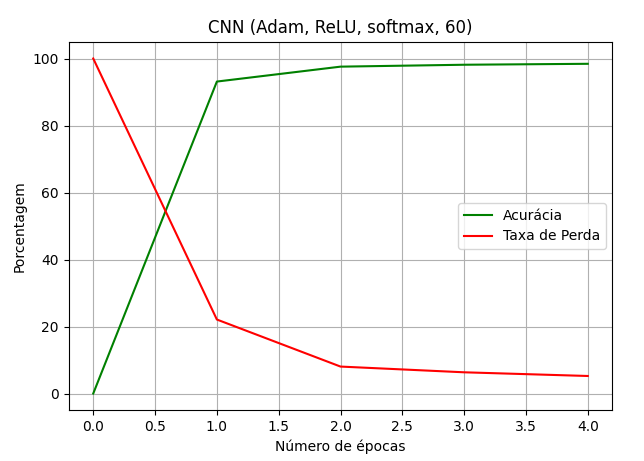
\includegraphics[width=.72\textwidth]{Images/cnn.png}
    \caption{Curva de aprendizado da CNN}
    \label{fig:exanpleFig1}
\end{figure}
\vspace*{-0.5cm}
\begin{figure}[H]
    \centering
    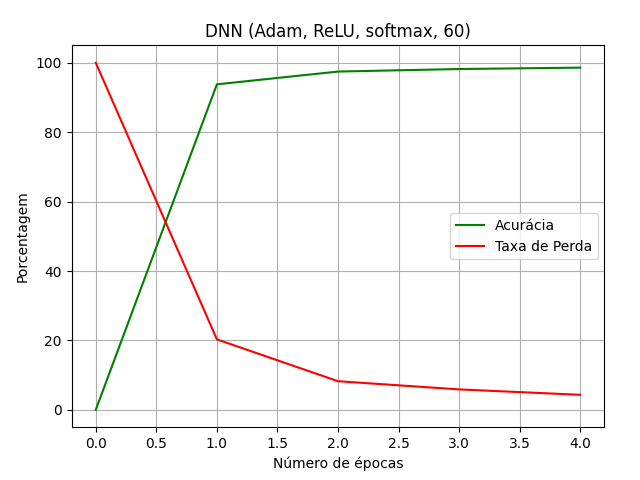
\includegraphics[width=.72\textwidth]{Images/dnn.png}
    \caption{Curva de aprendizado da DNN}
    \label{fig:exanpleFig2}
\end{figure}

\noindent A matriz de confusão obtida pelo modelo é exibida na Figura \ref{fig:exanpleFig3}.

\begin{figure}[H]
    \centering
    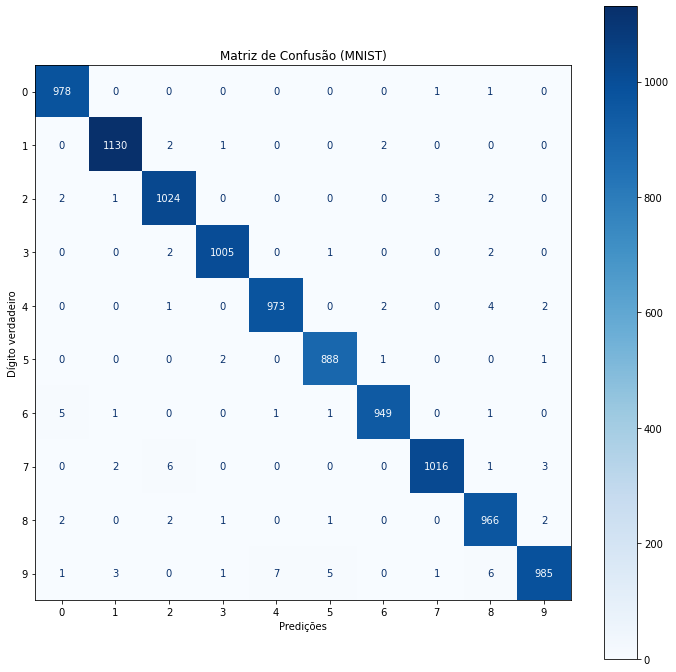
\includegraphics[width=.9\textwidth]{Images/confusion_matrix.png}
    \caption{Matriz de confusão da CNN}
    \label{fig:exanpleFig3}
\end{figure}

Nós tentamos formular nosso próprio conjunto de teste, escrevendo dígitos à mão e manipulando suas imagens para adequá-las à entrada das redes neurais, para que estas pudessem executar as predições. No entanto, as predições observadas foram bastante distantes das esperadas, dada a acurácia que as redes apresentaram e o padrão observado em suas predições errôneas.

Em um conjunto pequeno com apenas 13 imagens (Figura \ref{fig:exanpleFig4}), a CNN classificou a maioria como o dígito 3, embora a ocorrência do mesmo fosse única no conjunto. Na DNN, verificou-se o mesmo padrão, mas desta vez com o dígito 5, cuja ocorrência é verdadeira apenas em duas imagens. Os possíveis problema iniciais que pensamos que podem estar afetando as predições seriam os contornos dos dígitos, que não se apresentam de forma contígua e uniforme como na base de dados MNIST, além de ocuparem uma porção ligeiramente menor na imagem de dimensão 28 x 28. Estes são fatores de padronização que podem estar levando a classificação incorreta por parte das redes neurais, mas as causas também podem ser outras que ainda não conseguimos analisar.

\begin{figure}[H]
    \centering
    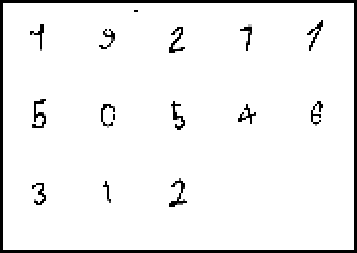
\includegraphics[width=.9\textwidth]{Images/instance.png}
    \caption{Conjunto de teste real}
    \label{fig:exanpleFig4}
\end{figure}

Embora a CNN tenha apresentado uma acurácia superior à observada na execução da DNN, consideramos que o custo de treinar uma rede neural convolucional não se mostra viável na aplicação para um problema de nicho simples como este. As diferenças entre as taxas de acurácia e perda entre ambas as redes é significativamente pequena, enquanto a disparidade entre seus tempos de execução é extremamamente alta, o que coloca a CNN em desvantagem na escolha de um modelo de aprendizado de máquina para a solução de tal problema.

\section{Considerações Finais}

Por fim, neste trabalho conseguimos explorar de forma bastante superficial, os conceitos por trás do subcampo da IA, o aprendizado de máquina e como construir modelos inteligentes que podem atuar de forma independente, analisando os mais diversos dados para nos fornecer soluções possíveis de serem obtidas por estes meios para alguns problemas do mundo real.

\section*{Referências}

\begin{itemize}
    \item Keras API reference: \url{https://keras.io/api/}
    \item Python \& NumPy utilities: \url{https://keras.io/api/utils/python_utils/#to_categorical-function}
    \item Layer activation functions: \url{https://keras.io/api/layers/activations/}
    \item Dense layer: \url{https://keras.io/api/layers/core_layers/dense/}
    \item Conv2D layer: \url{https://keras.io/api/layers/convolution_layers/convolution2d/}
    \item MaxPooling2D layer: \url{https://keras.io/api/layers/pooling_layers/max_pooling2d/}
    \item Optimizers: \url{https://keras.io/api/optimizers/}
    \item Losses: \url{https://keras.io/api/losses/}
    \item Ultimate Guide To Loss functions In Tensorflow Keras API With Python Implementation: \url{https://analyticsindiamag.com/ultimate-guide-to-loss-functions-in-tensorflow-keras-api-with-python-implementation/}
    \item Plotting Confusion matrix for tensorflow model: \url{https://www.kaggle.com/code/mdmashurshalehin/plotting-confusion-matrix-for-tensorflow-model/notebook}
    \item CNN | Introduction to Pooling Layer: \url{https://www.geeksforgeeks.org/cnn-introduction-to-pooling-layer/}
    \item Neural Network Optimization Algorithms: \url{https://towardsdatascience.com/neural-network-optimization-algorithms-1a44c282f61d}
    \item Image Thresholding: \url{https://docs.opencv.org/3.4/d7/d4d/tutorial_py_thresholding.html}
\end{itemize}

\end{document}
